% ||||||||||||||| <<<<< COMPILIEREN MIT pdflatex --shell-escape Dima-Hadoop-Vortrag.tex >>>>>> ||||||||||||||||||||||||||

\documentclass[hyperref={pdfpagelayout=SinglePage}]{beamer}

% ++++++++++++++++++++++++++++++++++++++++++++++++++++++++++++++++++ 
% +++ Theme ++++++++++++++++++++++++++++++++++++++++++++++++++++++++
% ++++++++++++++++++++++++++++++++++++++++++++++++++++++++++++++++++ 
\usetheme{dima}
\logo{
\includegraphics[width=1cm]{dimalogo.pdf}}

% ++++++++++++++++++++++++++++++++++++++++++++++++++++++++++++++++++ 
% +++ Positionierung und Beschriftung von Bildern ++++++++++++++++++
% ++++++++++++++++++++++++++++++++++++++++++++++++++++++++++++++++++ 
% enable eps graphic files
\usepackage[cleanup={log,aux,dvi,ps,pdf}]{auto-pst-pdf}
% enable absolute positioning on frames
\usepackage[absolute,overlay]{textpos}
% adjust the TPHorizModule and TPHorizModule units to the displayed mm grid Anzahl der horizontalen und vertikalen Linien des Beamer Grids
\TPGrid{13}{10}
% beschriftungen
\usepackage{overpic}
% grid for positioning \setbeamertemplate{background}[grid][step=1cm]

\usepackage{etex}
% ++++++++++++++++++++++++++++++++++++++++++++++++++++++++++++++++++ 
% +++ Encoding +++++++++++++++++++++++++++++++++++++++++++++++++++++
% ++++++++++++++++++++++++++++++++++++++++++++++++++++++++++++++++++ 
% verwende Vektorschriften, falls vorhanden
\usepackage[T1]{fontenc}

% Encodierung der Quelldatei latin1 = ISO 8859-1 ansinew = Windows applemac = Apple-Mac utf8 = UTF-8-Encoding
\usepackage[utf8]{inputenc}


% ++++++++++++++++++++++++++++++++++++++++++++++++++++++++++++++++++ 
% +++ Schriften ++++++++++++++++++++++++++++++++++++++++++++++++++++
% ++++++++++++++++++++++++++++++++++++++++++++++++++++++++++++++++++ 
% verwendete Schriften Doku:
% http://www.ctan.org/tex-archive/macros/latex/required/psnfss/psnfss2e.pdf
\usepackage{charter}
\usepackage[scaled=.92]{helvet}
\usepackage{courier}

% besseres Schriftbild Doku: http://www.ctan.org/tex-archive/macros/latex/contrib/microtype/microtype.pdf
\usepackage{microtype}


%++++++++++++++++++++++++++++++++++++++++++++++++++++++++++++++++++
%+++ Bilder +++++++++++++++++++++++++++++++++++++++++++++++++++++++
%++++++++++++++++++++++++++++++++++++++++++++++++++++++++++++++++++
% Für Floatobjekte
\usepackage{float}
% \FloatBarrier - Ermöglicht das forcierte Setzen von ausstehenden Floats. section macht vor jede section eine barrier.
\usepackage[section]{placeins} 

% Paket um Grafiken einbetten zu können
\usepackage{graphicx}
\graphicspath{{images/}}
\usepackage{subfigure}

% Zeilenumbruch bei Bildbeschreibungen.
%\setcapindent{1em}


%++++++++++++++++++++++++++++++++++++++++++++++++++++++++++++++++++
%+++ Sprache ++++++++++++++++++++++++++++++++++++++++++++++++++++++
%++++++++++++++++++++++++++++++++++++++++++++++++++++++++++++++++++
% neue Deutsche Rechtschreibung: Trennregeln!
\usepackage[english,german,ngerman]{babel}


%++++++++++++++++++++++++++++++++++++++++++++++++++++++++++++++++++
%+++ Literatur ++++++++++++++++++++++++++++++++++++++++++++++++++++
%++++++++++++++++++++++++++++++++++++++++++++++++++++++++++++++++++


\usepackage[
    backend=biber,
    url=true
]{biblatex}


\addbibresource{bib/references.bib}

%++++++++++++++++++++++++++++++++++++++++++++++++++++++++++++++++++
%+++ Verlinkung +++++++++++++++++++++++++++++++++++++++++++++++++++
%++++++++++++++++++++++++++++++++++++++++++++++++++++++++++++++++++
% Doku: http://www.ctan.org/tex-archive/macros/latex/contrib/hyperref/hyperref.pdf
%\usepackage[%
%pdfauthor={Erik Nijkamp and Alexander Alexandrov and Jan Marc Hoffmann},
%colorlinks, % verwende farbige Links
%linkcolor=blue, % Linkfarbe ist blau
%bookmarks, % erstelle Bookmarks der Links
%bookmarksopenlevel=1, % nur bis level 1 öffnen
%bookmarksopen, % Bookmarks werden beim öffnen des Dokumentes ebenfalls geöffnet
%urlcolor=blue, % Hyperlinks sind blau 
%citecolor=blue, % Cite Links sind blau
%bookmarksnumbered, % Bookmarks sind nummeriert
%final % Endversion 
%]{hyperref}

% fokusiert captions korrekt
%\usepackage[all]{hypcap}

\usepackage{listings}
% Listings Konfiguration
\lstset{language=Java, commentstyle=\color[RGB]{63,127,95}\ttfamily,
  keywordstyle=\color[RGB]{127,0,85}\bfseries,
  stringstyle=\color[RGB]{42,0,255}\ttfamily, showstringspaces=false,
  tabsize=2,
  % numbers=left,
  numberstyle=\tiny, numberblanklines=true, stepnumber=1,
  numbersep=5pt, xleftmargin=5pt,
  emphstyle=\color[RGB]{0,0,192}\texttt, breaklines=true,
  breakautoindent=true,
  % basicstyle=\tiny,
  extendedchars=true,
  % frame=shadowbox, rulesepcolor=\color{gray}
  %morekeywords={team,playedBy,as,when,after,before,base,within,replace,result,activate,deactivate}, %Erweiterung fuer Object Teams
  backgroundcolor=\color{white}, 
  framexleftmargin=2mm, 
  frame=shadowbox, 
  rulesepcolor=\color{lightgray}
}

% %%%%%%%%%%%%%%%%%%%%%%%%%%%%%%%%%%%%%%%%%%%%%%%%%%%%%%%% 
% Informationen zum Dokument
% %%%%%%%%%%%%%%%%%%%%%%%%%%%%%%%%%%%%%%%%%%%%%%%%%%%%%%%%

\author{\textcolor{gray}{Author:} Ward Schodts\\ \textcolor{gray}{Supervisor:}
Juan Soto}
\title{Pagerank in Apache Flink}
%s\subtitle{lll}
\institute{Datenbanksysteme und Informationsmanagement \\
Technische Universität Berlin \\[0.5cm]

\includegraphics[width=1.8cm]{tulogo}}
%\university{ss}
\date{\today}



% %%%%%%%%%%%%%%%%%%%%%%%%%%%%%%%%%%%%%%%%%%%%%%%%%%%%%%%% 
% Dokument 
% %%%%%%%%%%%%%%%%%%%%%%%%%%%%%%%%%%%%%%%%%%%%%%%%%%%%%%%%%

\begin{document}

% --------------------------------------------------------
\begin{frame}
\maketitle
\end{frame}
%--------------------------------------------------------

%--------------------------------------------------------
\begin{frame}
\frametitle{Agenda}
\tableofcontents
\end{frame}
%--------------------------------------------------------

% %%%%%%%%%%%%%%%%%%%%%%%%%%%%%%%%%%%%%%%%%%%%%%%%%%%%%%%% 
% Folien 
% %%%%%%%%%%%%%%%%%%%%%%%%%%%%%%%%%%%%%%%%%%%%%%%%%%%%%%%%%

\section{Introduction}

% --------------------------------------------------------------------------------------------------------------
\begin{frame}
\frametitle{Pagerank}
\begin{figure}
	\centering
	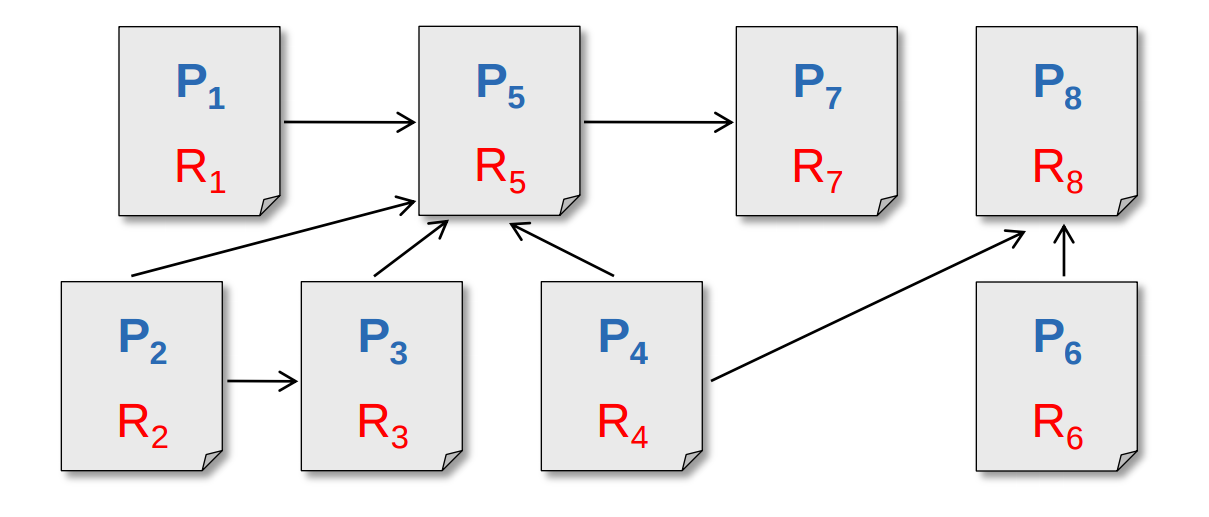
\includegraphics[width=0.8\textwidth]{pagerank1.png}
	\caption{PageRank example 1 \cite{prsigner}}
\end{figure}
\begin{itemize}
  \item A page has a high PageRank $R$ if
  \begin{itemize}
    \item there are many pages linking to it
    \item or, if there are some pages with a high PageRank
linking to it
  \end{itemize}
\end{itemize}
\end{frame}
% --------------------------------------------------------------------------------------------------------------

% --------------------------------------------------------------------------------------------------------------
\begin{frame}
\frametitle{Pagerank}

\begin{minipage}[l]{0.5\textwidth}
\textbf{$$ 
R(P_i)= \sum_{P_j \in B_i}\frac{R(P_j)}{L_j}
$$}
\begin{itemize}
  \item where
  \begin{itemize}
    \item $B_i$ is the set of pages that link to page $P_i$
    \item $L_j$ is the number of outgoing links for page $P_j$
linking to it
  \end{itemize}
\end{itemize}
\end{minipage}
\begin{minipage}[l]{0.49\textwidth}
\begin{figure}
	\centering
	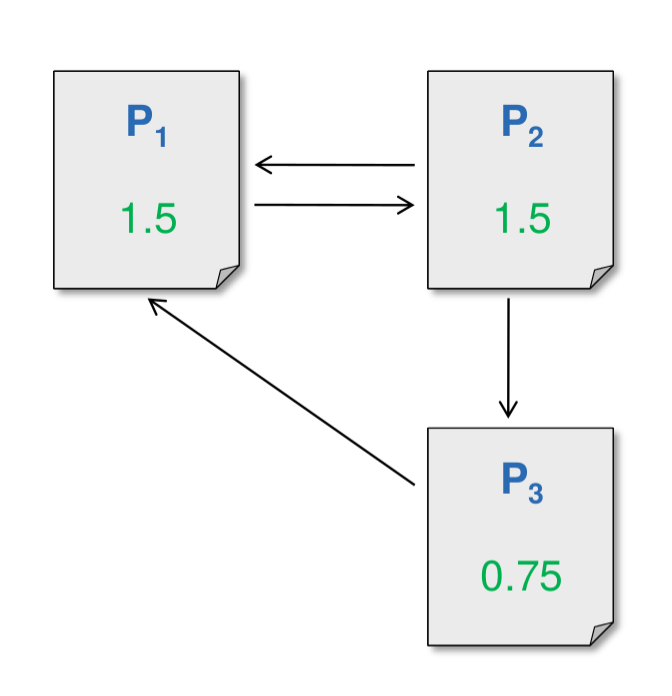
\includegraphics[width=\textwidth]{pagerank2.png}
	\caption{PageRank example 2 \cite{prsigner}}
\end{figure}
\end{minipage}

\end{frame}
% --------------------------------------------------------------------------------------------------------------

% --------------------------------------------------------------------------------------------------------------
\begin{frame}
\begin{figure}
	\centering
	
\includegraphics[width=0.65\textwidth]{squirrel.png}
	\caption*{\cite{squirrel}}
\end{figure}
\end{frame}
% --------------------------------------------------------------------------------------------------------------

% --------------------------------------------------------------------------------------------------------------
\begin{frame}
\frametitle{Apache Flink}
\begin{itemize}
\item Open source framework for distributed Big Data Analytics
\item Exploits:
	\begin{itemize}
	\item data streaming
	\item in-memory processing
	\item iteration operators
	\end{itemize}
to improve performance
\item Formerly Stratosphere (Flink means agile)
\item Developped here at TUB
\end{itemize}
\end{frame}
% --------------------------------------------------------------------------------------------------------------

% --------------------------------------------------------------------------------------------------------------
\begin{frame}
\begin{figure}
	\centering
	
\includegraphics[width=0.9\textwidth]{repetition.jpg}
	\caption*{\cite{repetition}}
\end{figure}
\end{frame}
% --------------------------------------------------------------------------------------------------------------

% --------------------------------------------------------------------------------------------------------------
\begin{frame}
\frametitle{Apache Flink: 2 possible setups}

\begin{minipage}[l]{0.5\textwidth}
\begin{figure}
	\centering
	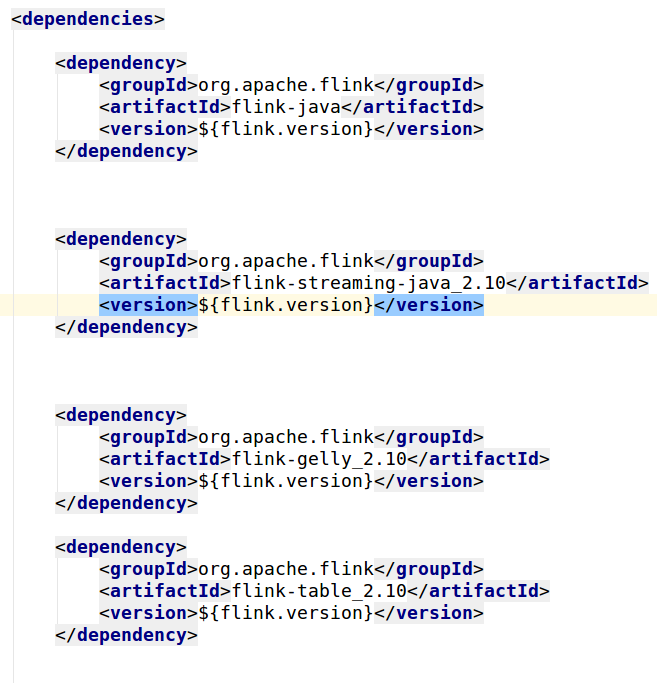
\includegraphics[width=0.9\textwidth]{pomxml.png}
	\caption{Maven}
\end{figure}
\end{minipage}
\begin{minipage}[l]{0.49\textwidth}
\begin{figure}
	\centering
	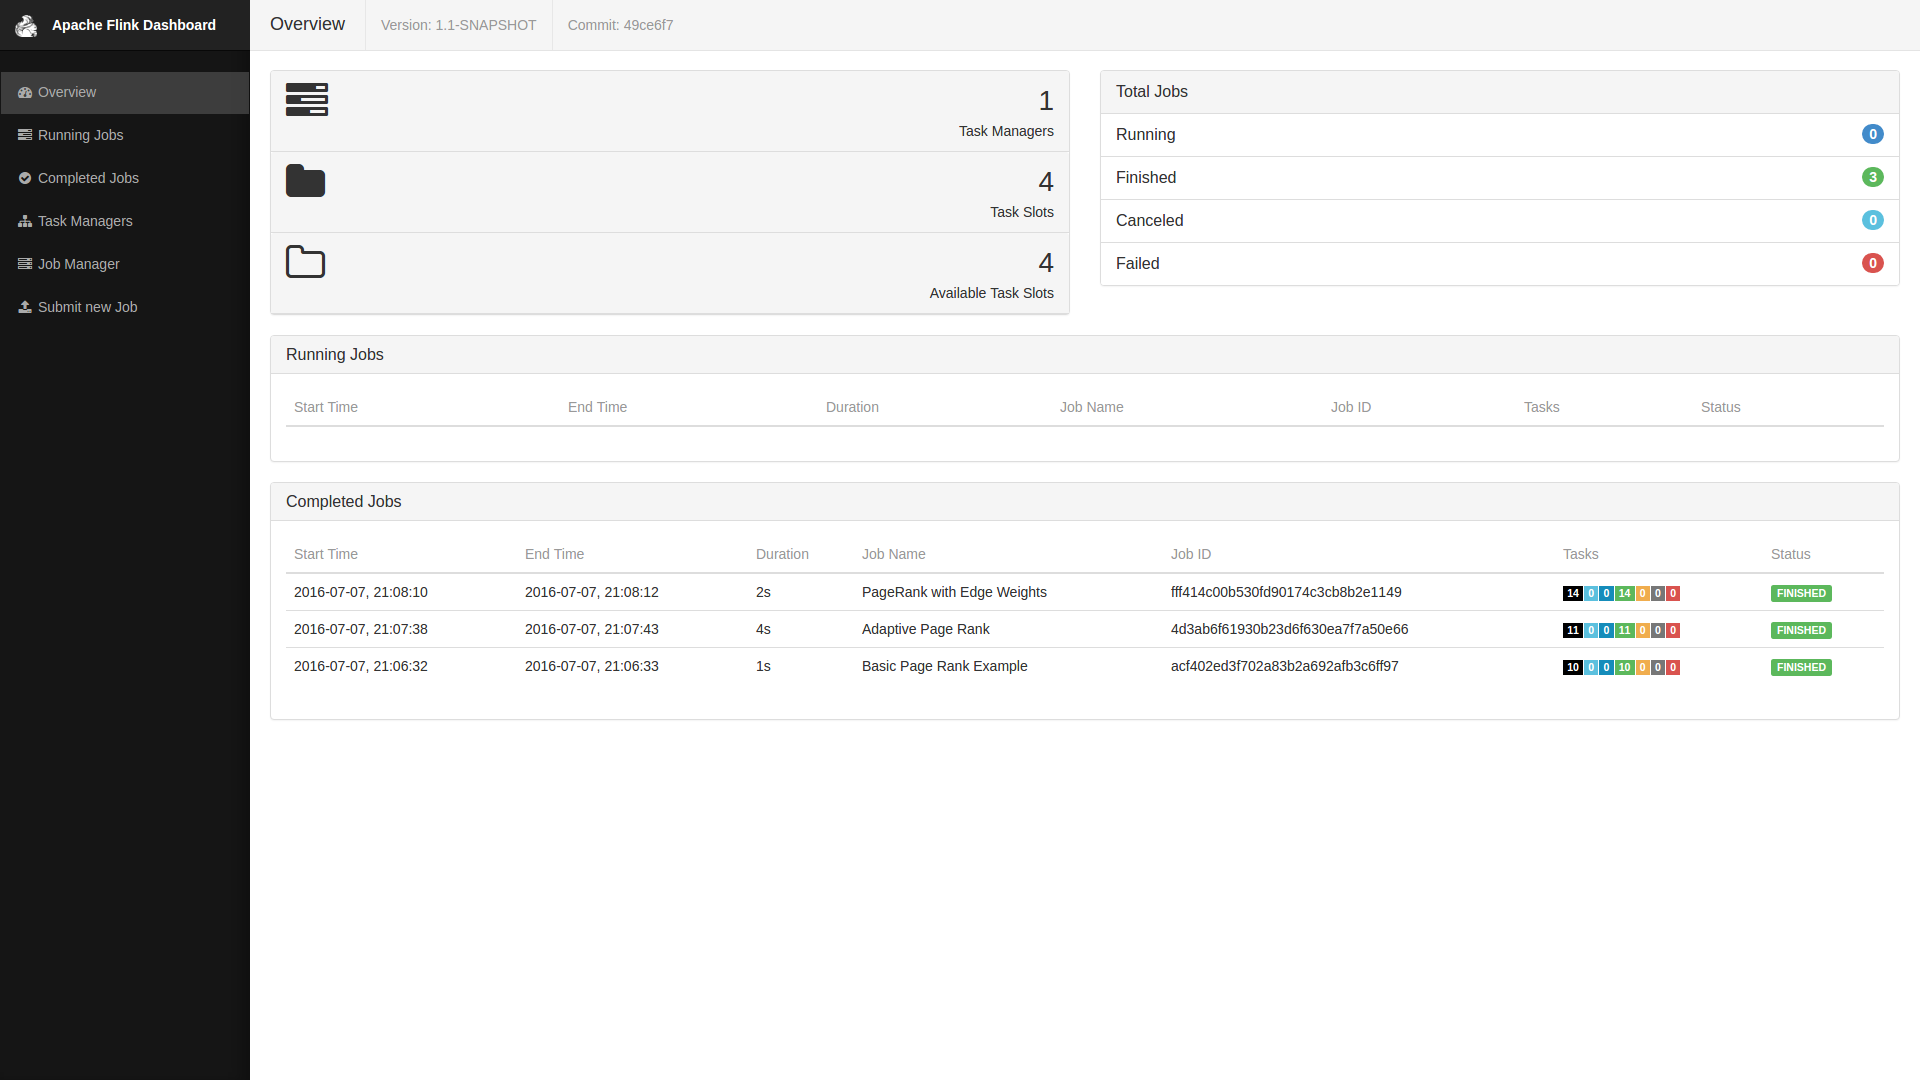
\includegraphics[width=\textwidth]{dashboard.png}
	\caption{Binary version (self compiled)}
\end{figure}
\end{minipage}
\end{frame}
% --------------------------------------------------------------------------------------------------------------

% --------------------------------------------------------------------------------------------------------------
\begin{frame}
\frametitle{Apache Flink: Gelly}

\begin{figure}
	\centering
	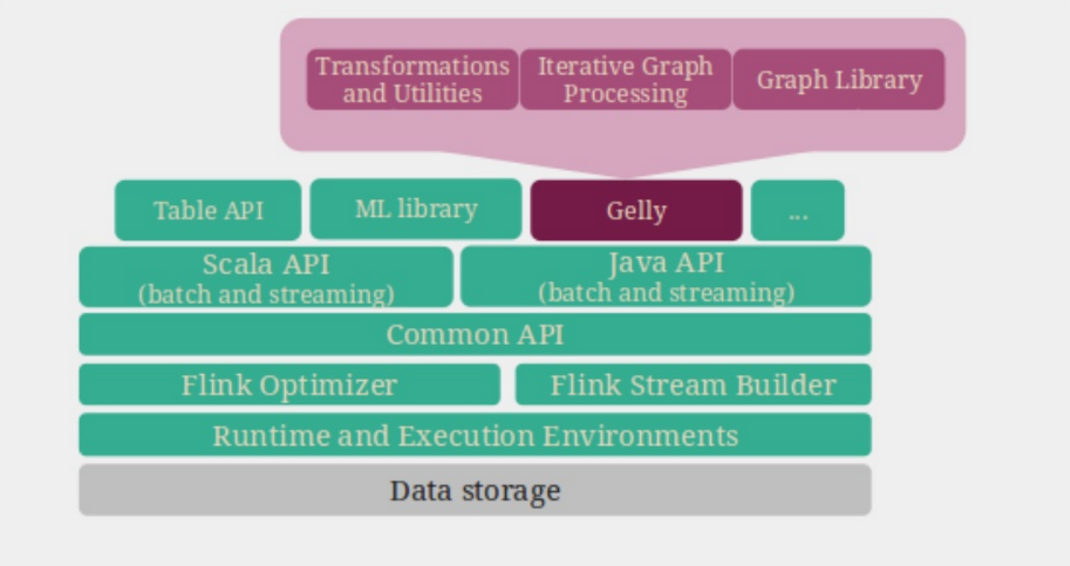
\includegraphics[width=\textwidth]{gelly.png}
	\caption{Gelly}
\end{figure}

\end{frame}
% --------------------------------------------------------------------------------------------------------------

% --------------------------------------------------------------------------------------------------------------
\begin{frame}
\frametitle{Apache Flink: Gelly}
\begin{itemize}
\item Large-scale graph processing API
\item On top of Flink's Java API
\item Off-the shelf library methods (e.g. pagerank)
\item Iterative algorithms
\end{itemize}


\end{frame}
% --------------------------------------------------------------------------------------------------------------

\section{The experiment}

% ------------------------------------------------------------------------------
\begin{frame}
\frametitle{Agenda}
\tableofcontents[currentsection]
\end{frame}
% ------------------------------------------------------------------------------

% ------------------------------------------------------------------------------
\begin{frame}
\frametitle{General experiment setup}
Experiment 1:
\begin{enumerate}
\item Data file with graph (and pagerank solution)
\item[] $\Downarrow$
\item Use Flink and Graphlab implemention to compute pagerank
\item[] $\Downarrow$
\item Compare with solution
\end{enumerate}

\end{frame}
% ------------------------------------------------------------------------------


% ------------------------------------------------------------------------------
\begin{frame}
\frametitle{General experiment setup}
Experiment 1:
\begin{enumerate}
\item Data file with graph (and pagerank solution)
\item[] $\Downarrow$
\item Use Flink and Graphlab implemention to compute pagerank
\item[] $\Downarrow$
\item Compare with solution
\end{enumerate}

Experiment 2:

\begin{enumerate}
\item Data file with huge graph (no solution yet)
\item[] $\Downarrow$
\item Use Flink and Graphlab implemention to compute pagerank
\item[] $\Downarrow$
\item Compare with each other
\end{enumerate}
\end{frame}
% ------------------------------------------------------------------------------

% ------------------------------------------------------------------------------
\begin{frame}
\frametitle{Experiment 1 data}
Data from a former Hadoop toolkit (Cloud9, now Bespin):
\begin{table}
\centering
\begin{tabular}{|c|c|c|}
\hline
Name & \# vertices & \# edges\\
\hline
Small & 93 & 195\\
\hline
Medium & 316 & 430\\
\hline
Large & 1458 & 3545\\
\hline
\end{tabular}
\end{table}
\end{frame}
% ------------------------------------------------------------------------------

% ------------------------------------------------------------------------------
\begin{frame}
\frametitle{Experiment 2 data}
Webgraph from \url{snap.stanford.edu/data/}
\begin{table}
\centering
\begin{tabular}{|c|c|c|}
\hline
Name & \# vertices & \# edges\\
\hline
web-Google & 875713 & 5105039\\
\hline
\end{tabular}
\end{table}
\end{frame}
% ------------------------------------------------------------------------------

\section{The different algorithm implementations}

% ------------------------------------------------------------------------------
\begin{frame}
\frametitle{Agenda}
\tableofcontents[currentsection]
\end{frame}
% ------------------------------------------------------------------------------


% ------------------------------------------------------------------------------
\begin{frame}
\frametitle{Flink algorithm 1}
\begin{figure}
	
	
\includegraphics[scale=0.2]{dataartisians.png}
	\caption{dataArtisans logo, \cite{artisians}}
\end{figure}
\begin{itemize}
\item An exercise from dataArtisans
\item Uses the standard Gelly implementation
\item \# input nodes = \# output nodes
\end{itemize}
\end{frame}
% ------------------------------------------------------------------------------

% ------------------------------------------------------------------------------
\begin{frame}
\frametitle{Flink algorithm 2}
\begin{figure}
	
	
\includegraphics[scale=0.2]{dataartisians.png}

\end{figure}

\begin{itemize}
\item A case study implementation from dataArtisans
\item A custom implementation
\item \# input nodes = \# output nodes
\end{itemize}
\end{frame}
% ------------------------------------------------------------------------------

% ------------------------------------------------------------------------------
\begin{frame}
\frametitle{Flink algorithm 3}
\begin{figure}

	
\includegraphics[scale=0.05]{squirrel.png}

\end{figure}

\begin{itemize}
\item An example from the Apache Flink repository
\item A custom implementation
\item \# input nodes != \# output nodes $\rightarrow$ filters
\end{itemize}
\end{frame}
% ------------------------------------------------------------------------------


% ------------------------------------------------------------------------------
\begin{frame}
\frametitle{Turi PageRank algorithm}
\begin{figure}
	\centering
	
\includegraphics[scale=0.5]{turi.png}
	\caption{Turi logo, \cite{turi}}
\end{figure}
\begin{itemize}
\item Used the standard implementation
\item Builds a graph out of the edges dataset
\end{itemize}


\end{frame}
% ------------------------------------------------------------------------------

% ------------------------------------------------------------------------------
\begin{frame}
\frametitle{Comparing the algorithms}
As part of the experimental setup, I implemented a test harness to compare the two PageRank solutions.
\begin{itemize}
	\item It can handle list of diffrence sizes.
	\item It takes care of equal PageRank values (they maybe sorted in different way).
	\item Has a modifiable window to compare solutions.
\end{itemize}
\end{frame}
% ------------------------------------------------------------------------------

\section{Results}

% ------------------------------------------------------------------------------
\begin{frame}
\frametitle{Agenda}
\tableofcontents[currentsection]
\end{frame}
% ------------------------------------------------------------------------------


% ------------------------------------------------------------------------------
\begin{frame}
\frametitle{Results: experiment 1}
\LARGE Any expectations?
\end{frame}
% ------------------------------------------------------------------------------

% ------------------------------------------------------------------------------
\begin{frame}
\frametitle{Results: experiment 1}
\begin{figure}

	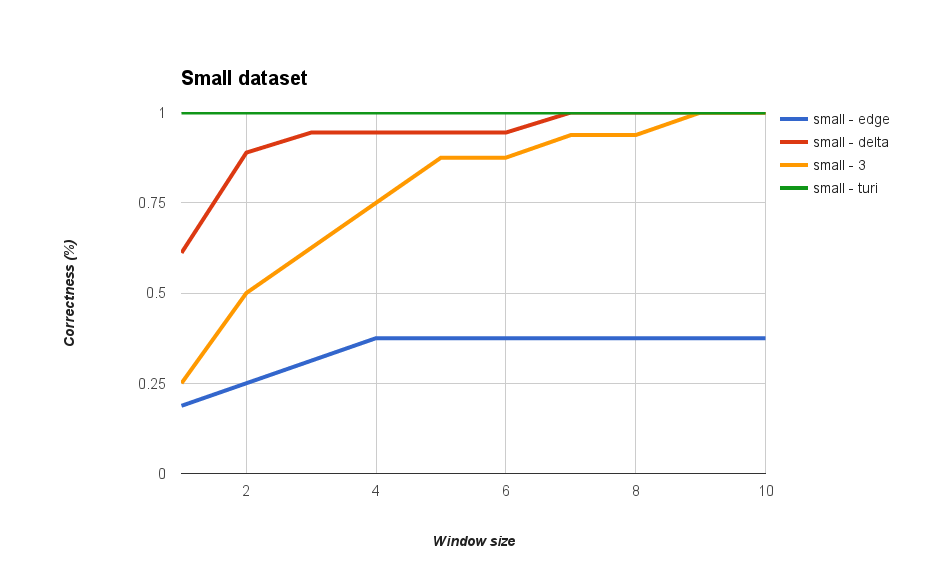
\includegraphics[width=\textwidth]{small.png}

\end{figure}
\end{frame}
% ------------------------------------------------------------------------------

% ------------------------------------------------------------------------------
\begin{frame}
\frametitle{Results: experiment 1}
\begin{figure}

	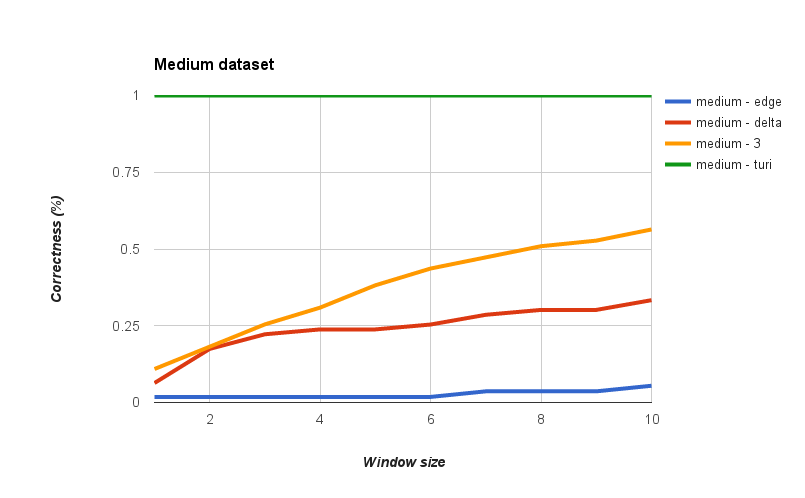
\includegraphics[width=\textwidth]{medium.png}

\end{figure}
\end{frame}
% ------------------------------------------------------------------------------

% ------------------------------------------------------------------------------
\begin{frame}
\frametitle{Results: experiment 1}
\begin{figure}

	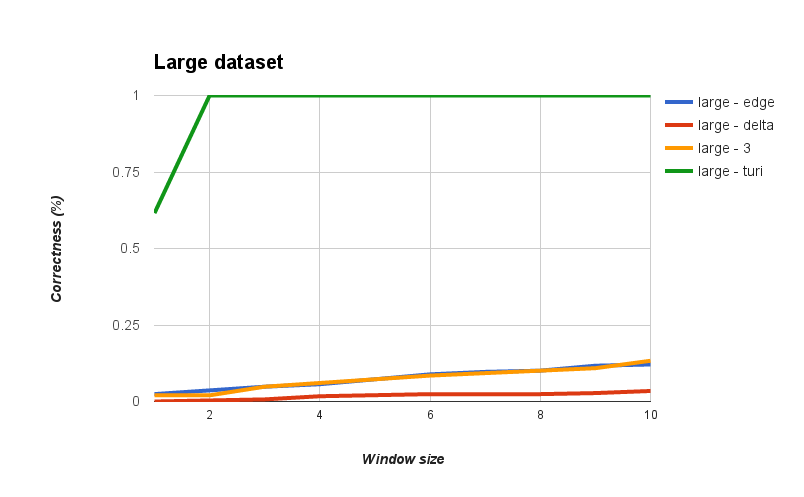
\includegraphics[width=\textwidth]{large.png}

\end{figure}
\end{frame}
% ------------------------------------------------------------------------------

% ------------------------------------------------------------------------------
\begin{frame}
\LARGE These results are ...?
\end{frame}
% ------------------------------------------------------------------------------

% ------------------------------------------------------------------------------
\begin{frame}
\frametitle{Why are the results so bad?}
\LARGE ... Bad
\end{frame}
% ------------------------------------------------------------------------------
% ------------------------------------------------------------------------------
\begin{frame}
\frametitle{Why are the results so bad?}
\LARGE Any ideas?
\end{frame}
% ------------------------------------------------------------------------------

% ------------------------------------------------------------------------------
\begin{frame}
\frametitle{Why are the results so bad?}
\begin{figure}

	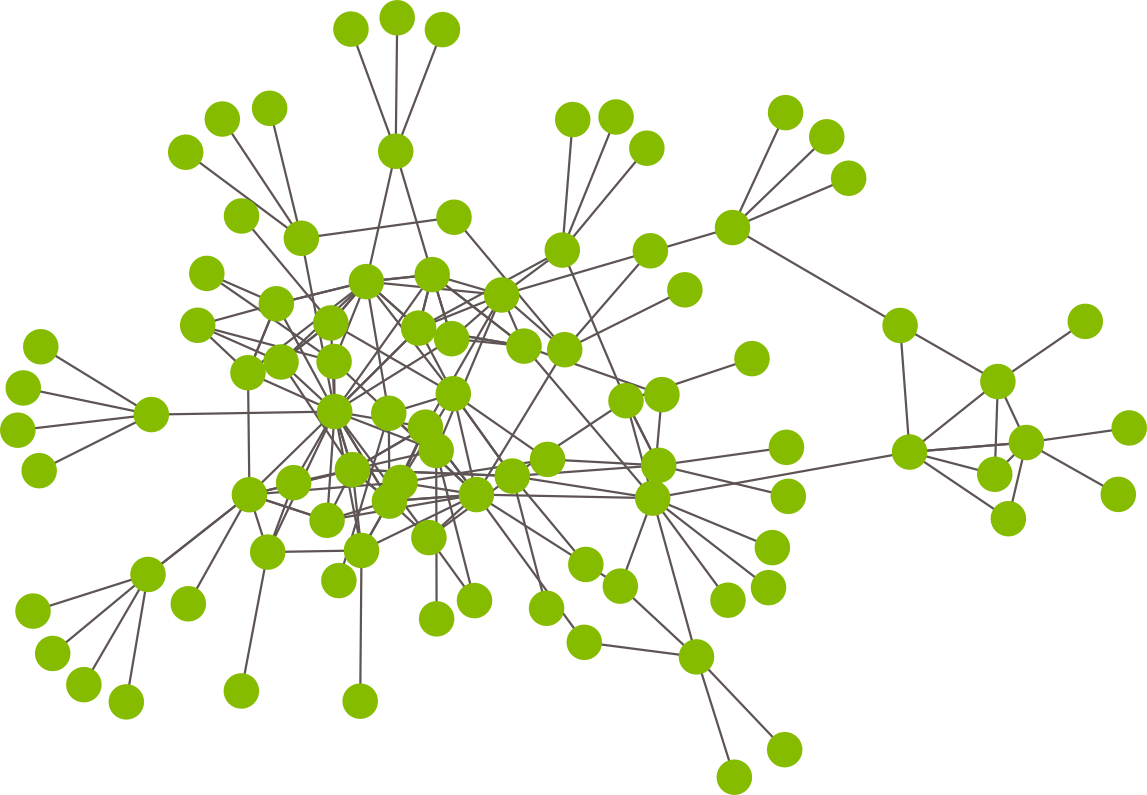
\includegraphics[width=\textwidth]{smallgraph.png}

\end{figure}
\end{frame}
% ------------------------------------------------------------------------------

% ------------------------------------------------------------------------------
\begin{frame}
\frametitle{Why are the results so bad?}
\begin{figure}

	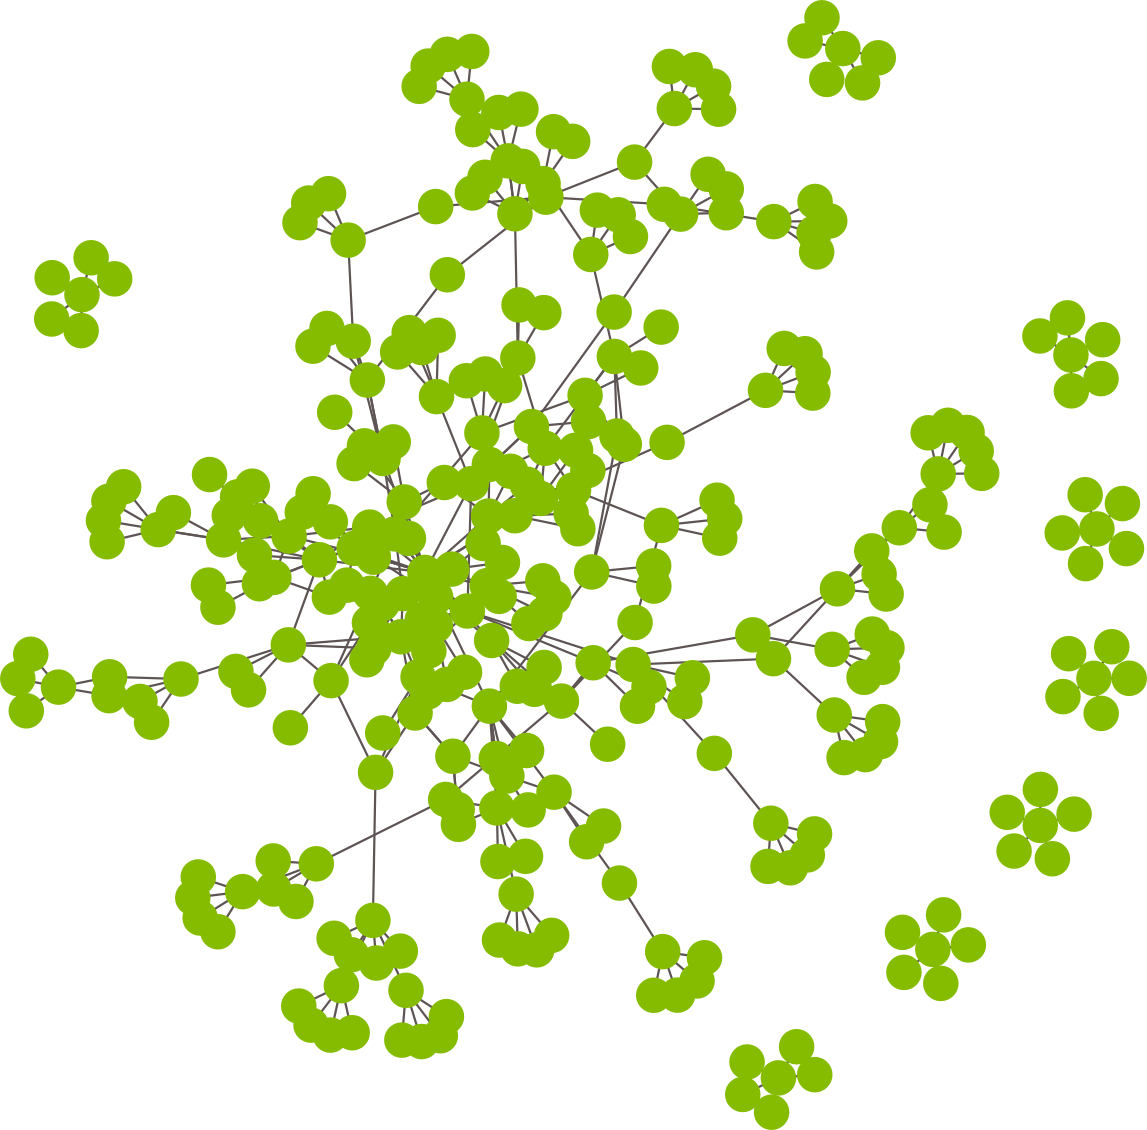
\includegraphics[width=0.7\textwidth]{mediumgraph.png}

\end{figure}
\end{frame}
% ------------------------------------------------------------------------------

% ------------------------------------------------------------------------------
\begin{frame}
\frametitle{Why are the results so bad?}
\begin{figure}

	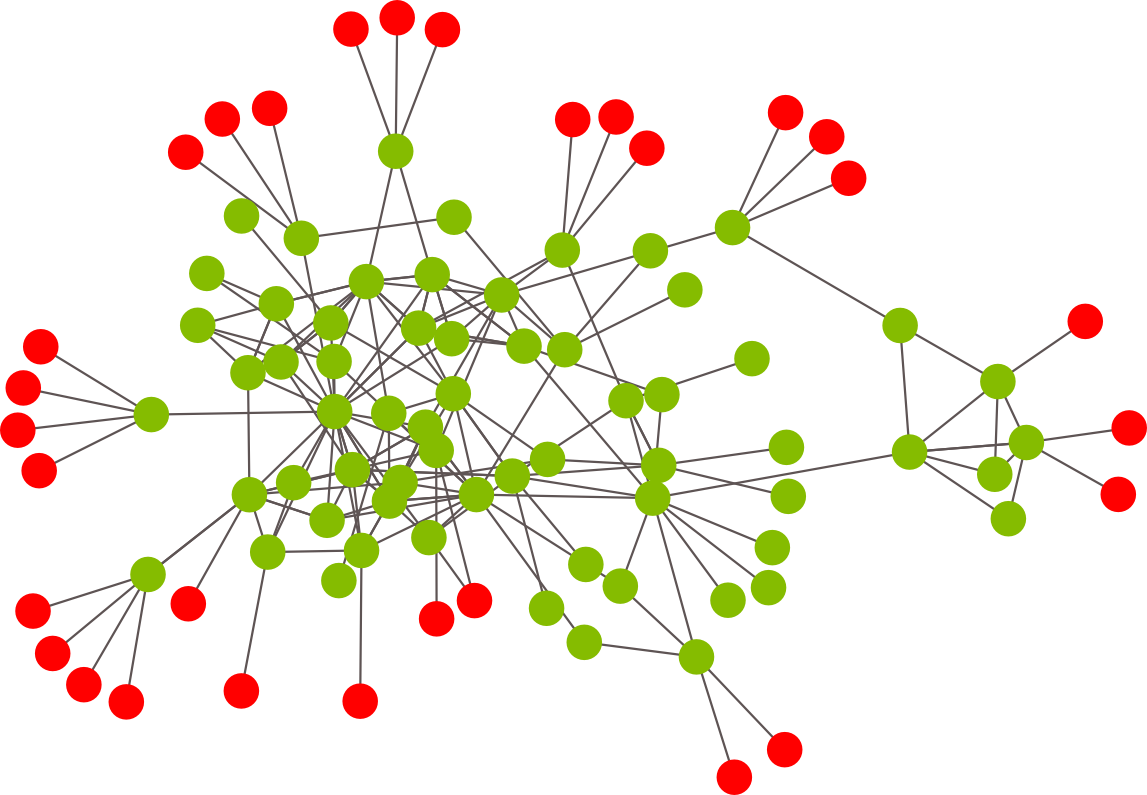
\includegraphics[width=\textwidth]{smallredgraph.png}

\end{figure}
\end{frame}
% ------------------------------------------------------------------------------

% ------------------------------------------------------------------------------
\begin{frame}
\frametitle{Why are the results so bad?}
\begin{figure}

	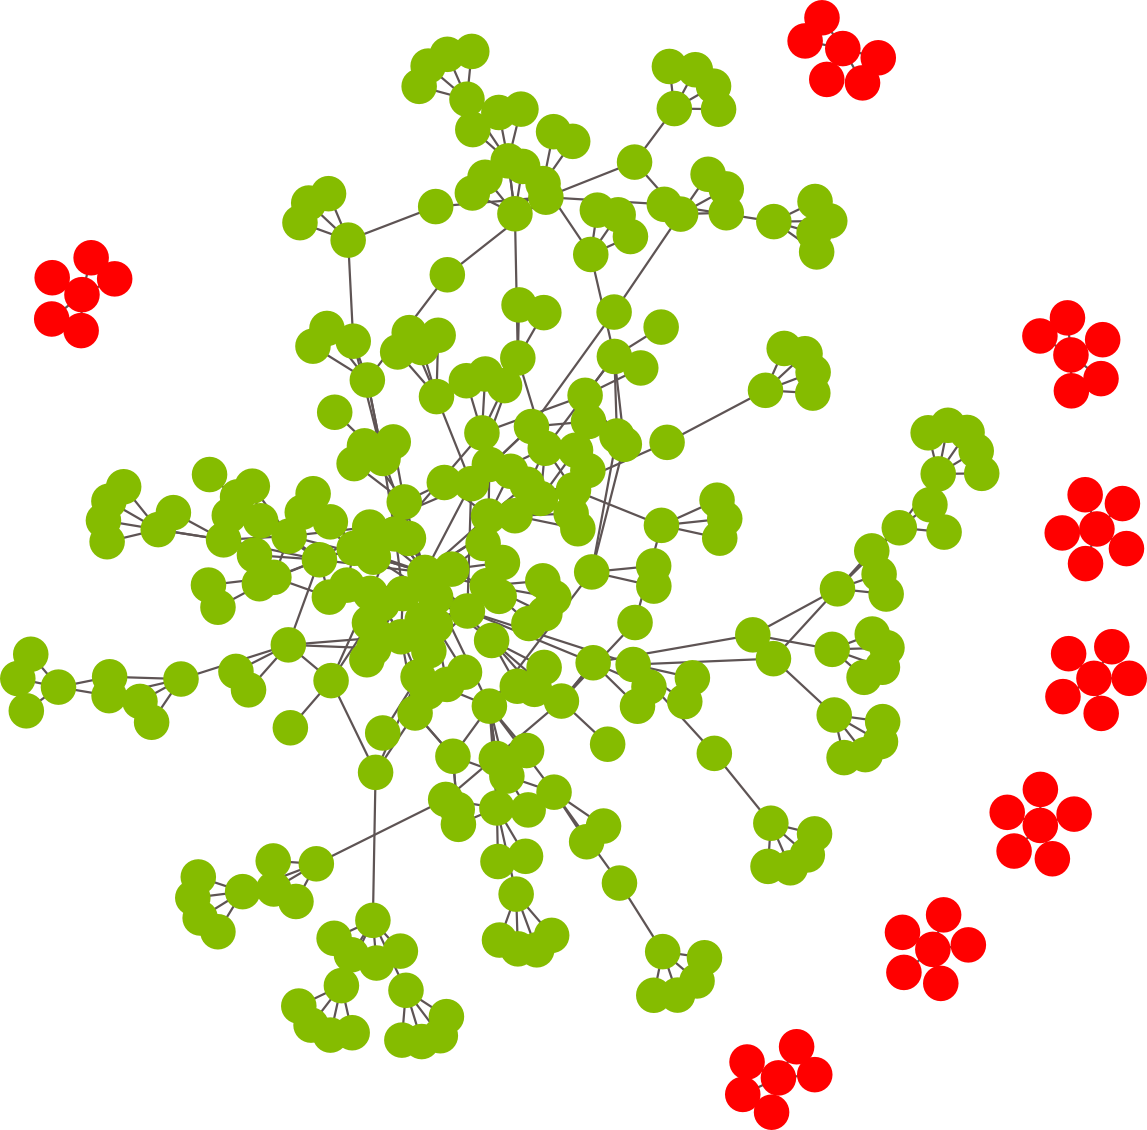
\includegraphics[width=0.7\textwidth]{mediumredgraph.png}

\end{figure}
\end{frame}
% ------------------------------------------------------------------------------


% ------------------------------------------------------------------------------
\begin{frame}
\frametitle{Why are the results so bad?}
\begin{itemize}
\item Implementations expext an incoming and outging edge for every node
\item Dangling nodes
\item Spider traps
\end{itemize}

$\rightarrow$ they are all basic implementations\\
$\rightarrow$ Turi has a advanced implementation
\end{frame}
% ------------------------------------------------------------------------------


% ------------------------------------------------------------------------------
\begin{frame}
\frametitle{Speed of experiment 1}
\begin{figure}

	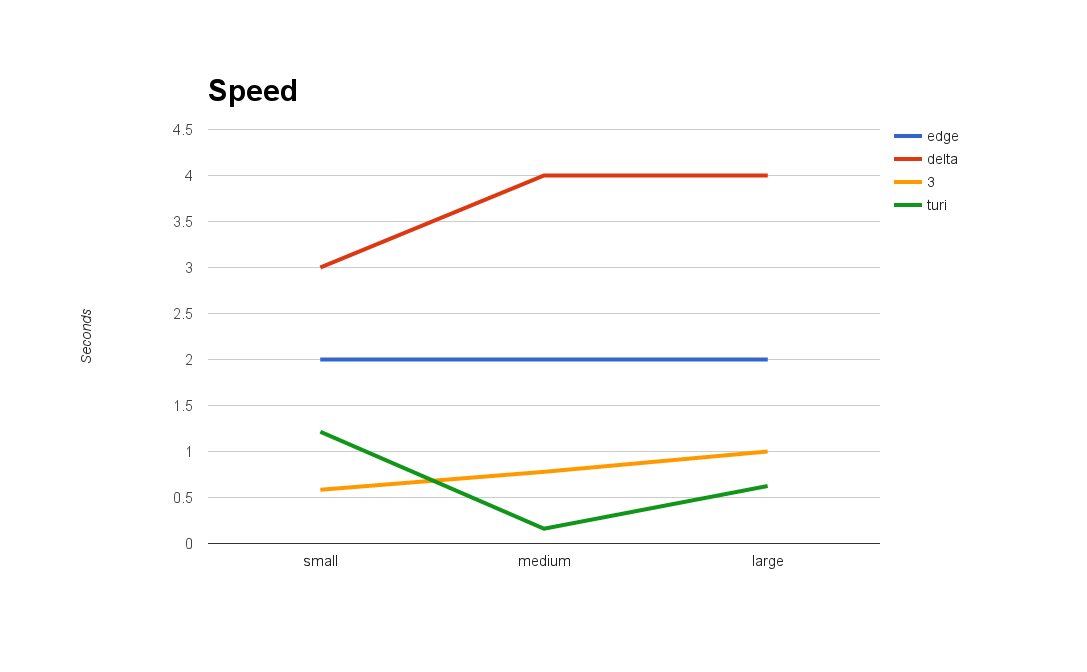
\includegraphics[width=0.9\textwidth]{speeds.png}

\end{figure}
$\rightarrow$ no huge differences with Turi
\end{frame}
% ------------------------------------------------------------------------------

\begin{frame}
\frametitle{Experiment 2}
\begin{figure}

	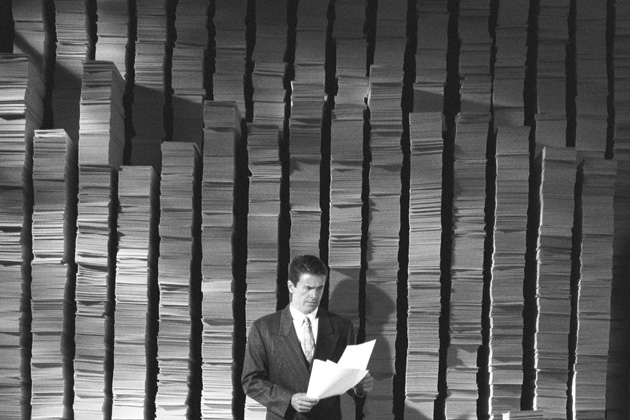
\includegraphics[width=0.9\textwidth]{huge.jpg}

\end{figure}

\end{frame}

% ------------------------------------------------------------------------------
\begin{frame}
\frametitle{Speed of experiment 2}
\begin{table}
\centering
\begin{tabular}{|c|c|c|c|c|}
\hline
Algorithm & Edge & Delta & 3 & Turi\\
\hline
Time (s) & 633 & 549 & 14 & 45\\
\hline
\end{tabular}
\end{table}

\begin{itemize}
\item First two algortihms are a lot slower $\backsim$ 10 times.
\item Algorithm 3 cheats with the filtering
\end{itemize}

\end{frame}
% --

% ------------------------------------------------------------------------------
\begin{frame}

\begin{figure}

	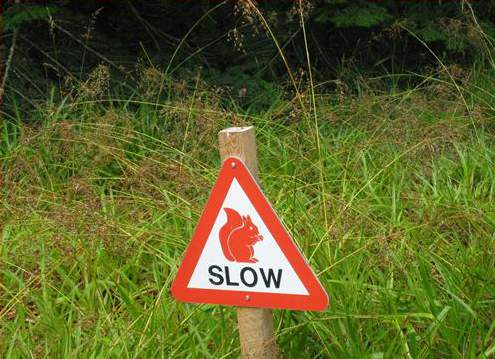
\includegraphics[width=\textwidth]{slow.jpg}

\end{figure}
\end{frame}
% ------------------------------------------------------------------------------


% ------------------------------------------------------------------------------
\begin{frame}
\frametitle{Speed of experiment 2}
\begin{figure}

	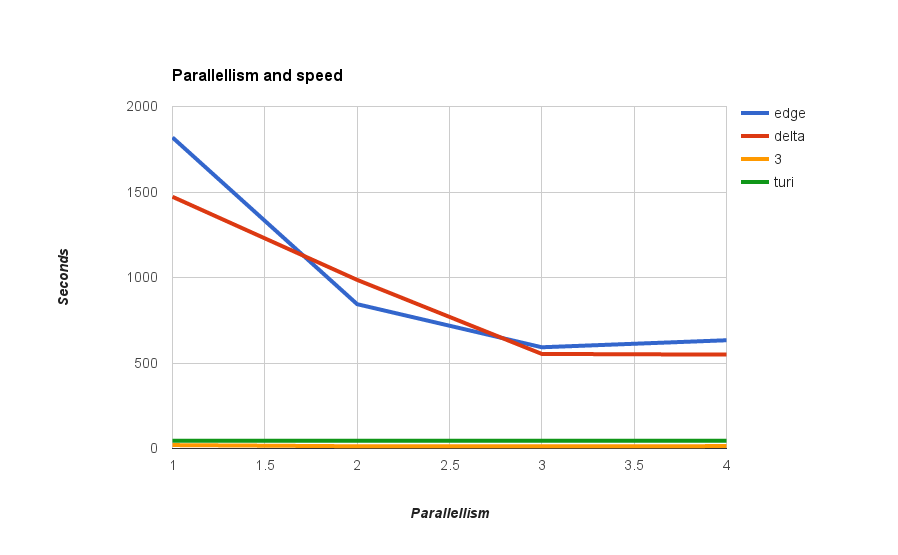
\includegraphics[width=\textwidth]{parallellism.png}

\end{figure}
\end{frame}
% ------------------------------------------------------------------------------


\section{Conclusion}
% ------------------------------------------------------------------------------
\begin{frame}
\frametitle{Agenda}
\tableofcontents[currentsection]
\end{frame}
% ------------------------------------------------------------------------------

% ------------------------------------------------------------------------------
\begin{frame}
\frametitle{Conclusion}

\end{frame}
% ------------------------------------------------------------------------------


%--------------------------------------------------------
\begin{frame}
\frametitle{Vielen Dank für Ihre Aufmerksamkeit}
\begin{center}
{\LARGE Fragen?}
\end{center}



\end{frame}

\begin{frame}[allowframebreaks]
		
        \frametitle{References}
        \nocite{*}
        \printbibliography

\end{frame}
%--------------------------------------------------------

\end{document}
